\section{Introduction}
\label{sec:intro}

Real-time object detection on embedded GPUs is usually evaluated with
two numbers per model: COCO accuracy~\cite{lin2014coco} and the latency
of the compiled engine in an isolated benchmark. Efficiency research
therefore focuses on the model: structured
pruning~\cite{li2017pruning,fang2023depgraph},
quantization-aware training~\cite{jacob2018quantization} and
distillation~\cite{hinton2015distilling} are judged by the engine
latency they remove per unit of accuracy lost. NMS-free detectors
make this framing seem even more natural. YOLOv10~\cite{wang2024yolov10}
and YOLO26~\cite{jocher2026yolo26,ultralytics2026yolo26} emit a fixed set of final detections
from a one-to-one head, so the host only decodes the image and converts
a few hundred output rows. With post-processing nearly gone, the engine
benchmark should predict the application.

\begin{figure*}[pos=t]
\centering
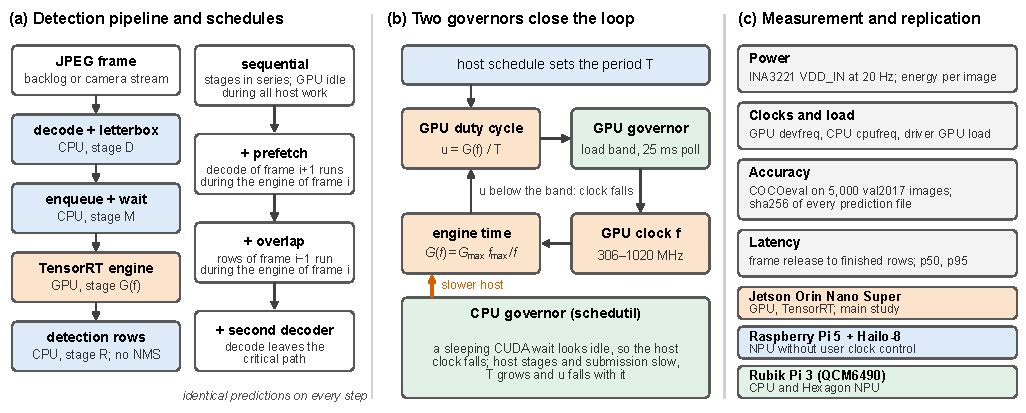
\includegraphics[width=\textwidth]{figs/framework.pdf}
\caption{Overview of the study. (a) The detection pipeline, with the
stage symbols of \cref{sec:sysmodel}, and the cumulative schedule
ladder of \cref{sec:ladder}; every scheduling step keeps the predictions
byte-identical. (b) The feedback loop described by the duty-cycle
model. The host schedule sets the period $T$ and thus the GPU duty
cycle $u$. When $u$ lies below the governor's load band, the GPU clock
falls and engine time grows. A sleeping CUDA wait also lets the CPU
governor lower the host clock, which lengthens $T$. (c) Quantities
measured on every run and the three boards of the study
(\cref{sec:setup,sec:crossplatform}).}
\label{fig:framework}
\end{figure*}

Measurements on an NVIDIA Jetson Orin Nano Super show that it does not.
Run back-to-back, the FP16 TensorRT engine of YOLO26n takes 4.2\,ms per
inference. In a conventional sequential application that decodes a
JPEG, letterboxes it, runs the engine and builds detection rows, the
same engine takes 13.2\,ms. The model, input and builder are unchanged;
the GPU's duty cycle is not. While the CPU decodes, the GPU idles, and
the stock frequency governor holds the GPU at its minimum clock of
306\,MHz, 30\% of its maximum. This also affects how compression
should be judged. A model 20\% cheaper in the benchmark would gain
little in such an application: at a fixed clock the saving is diluted
by the host stages, and the clock itself does not move.

The study did not start with governors. It first tried to make YOLO26n
cheaper through object-aware structured pruning, quantization-aware
training (QAT), distillation, compiler-guided pruning of the most
expensive head layers, and a per-image adaptive-resolution router.
These variants either lost several AP points or did not run faster once
compiled, and the router failed verification on held-out images. Only the
host pipeline was then restructured. Under the same default governors and with byte-identical
predictions, this gave $2.4\times$ the throughput of the best
sequential pipeline, even with all of that pipeline's clocks locked at
maximum. The gain over the standard Ultralytics predictor was
$6.9\times$.

This paper is a systematic measurement study of that gap, guided by
five research questions:
\begin{itemize}
\item[\RQ{1}] How does the GPU governor's response to an application's
  duty cycle determine the in-application cost of a fixed engine, and
  can a simple model describe it?
\item[\RQ{2}] Which host-pipeline decisions matter for throughput and
  energy, how large is each effect, and which of them interact with the
  governor?
\item[\RQ{3}] How do these decisions trade latency against energy when
  frames arrive at camera rates rather than as a backlog?
\item[\RQ{4}] How do model-level decisions (input resolution,
  compression, model size) rank once the pipeline is fixed?
\item[\RQ{5}] Do the findings carry over to other NMS-free detectors
  and to other accelerator architectures?
\end{itemize}

\noindent The contributions are:
\begin{enumerate}
\item A duty-cycle model of in-application engine time and energy
  (\cref{sec:sysmodel}), checked against direct measurements
  (\cref{sec:diagnosis}). Engine time scales with the inverse of the
  measured clock. The driver-reported GPU load is consistent with a
  load-band governor whose observed band is schedule-specific. A
  sequential pipeline sits at or below the top of that band even at the
  minimum clock, which is consistent with its never leaving the floor.
  Splitting energy into an idle floor and a marginal term gives an
  empirical upper envelope for the measured below-capacity streaming
  cells (\cref{sec:stream}).
\item A controlled, cumulative pipeline ablation on all 5,000 COCO
  val2017 images (\cref{sec:ladder}). Scheduling variants produce
  byte-identical predictions, so accuracy is held exactly constant.
  Each variant is reported with official COCO AP, throughput, input
  energy, GPU clock and CPU time under both default and locked clocks,
  and the number of decode workers is swept. On the sequential and
  prefetch schedules, the choice between two CUDA synchronization calls
  costs 17--20\% of throughput under the default governors. This loss
  is governor-mediated and drops below 1\% with locked clocks. On the
  full two-worker schedule the wait policy itself is free: a sleeping
  event wait matches a spinning one within 1\% under default and locked
  clocks. The 24\% that stream synchronization still costs there is a
  completion-boundary effect, identical at locked clocks. A controlled
  test traces the governor-mediated loss to the CPU governor: a
  sleeping wait lets \texttt{schedutil} lower the clock of the host's
  frequency domain. Keeping that domain busy recovers 97\% of the loss.
  A per-task utilization clamp~\cite{linux2024uclamp}, set without root
  privileges, recovers most of it at lower energy. Garbage-collection
  pauses in a typical evaluation loop also cost a fast pipeline 7.1\%
  of its measured throughput.
\item A streaming evaluation at 15, 30 and 60\,fps (\cref{sec:stream}).
  Energy per frame is set mainly by idle power. The highest-throughput
  configuration adds one frame period of latency at low rates. An
  arrival-aware variant removes this cost and keeps p95 latency at or
  below 41\,ms at all three rates.
\item An evaluation of model-level decisions under a fixed, optimized
  pipeline (\cref{sec:model}). Lower input resolution buys 27\% throughput in
  a naive pipeline but only 2--4\% in an optimized one (6--10\% with
  Python's cyclic garbage collector disabled). The compression and
  routing attempts are reported as negative results. On YOLO26s and
  YOLOv10n, the pipeline effects are comparable to YOLO26n's
  ($5.6$--$6.9\times$ over the standard predictor).
\item A replication of the core experiments on two further boards
  (\cref{sec:crossplatform}): a Raspberry Pi~5 with a Hailo-8 NPU,
  whose accelerator has no user-visible frequency control, and a Rubik
  Pi~3 (Qualcomm QCM6490), measured on both its CPU and its Hexagon
  NPU. The pipeline ladder transfers ($3.3\times$ on the Pi~5 with
  byte-identical predictions, $2.7\times$ before the wait-policy
  change). The Jetson-specific accelerator-governor signature is not
  directly observed on the NPU stacks, where the identifiable mechanisms
  shift to the host side. With CPU inference, the ladder flattens and
  sustained load becomes thermally limited. On the NPU stack, the CPU
  governor becomes the largest term (57\% on the matched overlap rungs)
  because the scheduler down-clocks the core that feeds the
  accelerator. That core falls from 2.7\,GHz (pinned) to
  0.95--1.8\,GHz, depending on how little host work the schedule leaves
  on the critical path.
\end{enumerate}

\Cref{fig:framework} gives an overview of the pipeline, the feedback
loop and the measurement setup. This paper does not propose a new
detector, compression method or governor, and pipelining itself is
standard practice. Its contribution
is the measurement and its explanation. On this class of device, the
interaction between the host pipeline and the frequency governor
determines more of the end-to-end cost than the model-level choices
that usually receive attention. All scripts, raw power traces and
prediction hashes are provided for checking and reproduction (see the
data and code availability statement).
